\section{Installation and Architecture}
\label{sec.install}

This section presents an overview of the installation procedure and
the distributed architecture of $\pvslm$.

The $\pvslm$ tool can be installed automatically from the command line
by issuing the following command:
%
\begin{verbatim}
  curl http://migueleci.github.io/pvslm/downloads/pvslm-conf.py \
    -o pvslm-install && chmod +x pvslm-install && \
    python ./pvslm-install
\end{verbatim}
%
This command uses the $\curl$ utility to download the $\pvslm$
installation sources from GitHub. Once these sources are downloaded
and some file permissions adjusted, the installation process is
executed as a Python 2 script. During the installation process, the
user can select the location in which the tool is to be installed,
including where the configuration files for the library sources and
the local copy of the libraries are to be placed. This script has been
tested both on Linux and Mac OS X boxes. Figure~\ref{fig.install}
depicts a successful installation procedure of $\pvslm$ in a Ubuntu
Linux box.

\begin{figure}
  \centering
  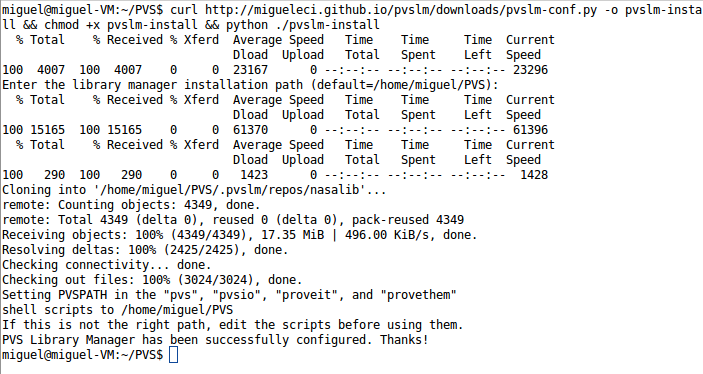
\includegraphics[width=11cm]{images/install.png}
  \caption{A successful installation procedure of $\pvslm$ in a Ubuntu
    Linux box.}
  \label{fig.install}
\end{figure}

Upon its successful installation, $\pvslm$ automatically configures
the NASALib library sources and makes a local copy of them by using
Git's clone command, so they are available for installation in PVS.

The $\pvslm$ tool is desiged with a distributed architecture. It can
connect to library sources over the internet. Each time a source is
configured, $\pvslm$ can download the library into the host system as
a local $\git$ repository. Further updates of the library are carried
out internally by $\pvslm$ by using $\git$'s pull
command. Figure~\ref{fig.arch} depicts the architecture of
$\pvslm$. It is important to note that although GitHub is used as
$\git$ server of reference throughout this paper, it is also possible
to use other publicly available servers such as BitBucket, for
instance, containing an annotated library.

\begin{figure}
  \centering 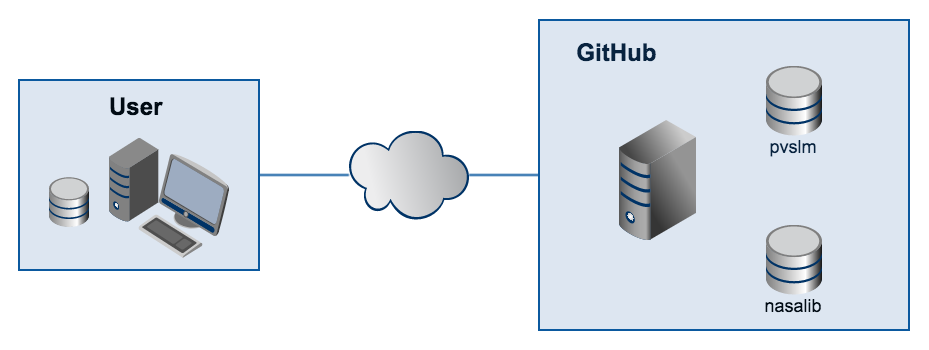
\includegraphics[width=11cm]{images/arch.png}
  \caption{Distributed architecture of $\pvslm$.}
  \label{fig.arch}
\end{figure}
